\section{Sampling Metodları}
Veri analizi ve makine öğrenimi projelerinde, dengesiz veri setleri sıkça karşılaşılan bir sorundur. Özellikle sınıflandırma problemlerinde, nadir sınıfların fazla sınıflara göre daha az örneklenmiş olması, modelin yanlış sonuçlar üretmesine neden olabilir. İşte bu durumda, oversampling ve undersampling gibi teknikler devreye girer.

Oversampling, nadir sınıflara ait örnekleri çoğaltarak veya yeniden örnekleme yaparak veri setinin dengesini sağlama işlemidir. Bu yöntem, nadir sınıfların temsil edilme oranını artırarak modelin daha dengeli bir şekilde eğitilmesini sağlar. Undersampling, fazla sınıflara ait örnekleri azaltarak veya örnekleri rastgele seçerek veri setinin dengesini sağlama işlemidir. Bu yöntem, fazla sınıfların temsil edilme oranını azaltarak veri setini daha dengeli hale getirir. Undersampling, modelin dengeli bir şekilde eğitilmesini sağlayabilir, ancak nadir sınıfların temsil edilme oranını azaltma riski taşır.

\begin{itemize}
    \item Dengesiz sınıf dağılımı düşük tespit oranına (recall score) yol açar.
    \item Örneklem arttırma (oversampling), örneklem azaltma (undersampling)
    \item Çoğunluk (majority), azınlık (minority)
\end{itemize}

Under Sampling Metodları
\begin{enumerate}
    \item Dönüştürülmüş Veri Seti Üzerinden Örneklem Seçen Metodlar
    \begin{enumerate}
        \item \textbf{Near Miss Undersampling:} Çoğunluk sınıfın azınlık sınıflara uzaklığına göre bu örneklemleri seçen bir örneklem azaltma metodudur.
        \item \textbf{Condensed Nearest Neighbors Rule:} CNN, KNN algoritmasının memory ihtiyacını azaltması için üretildi.
    \end{enumerate}
    \item Silinecek Örnekleri Seçen Metodlar
    \begin{enumerate}
        \item \textbf{Tomek Links:} Her bir sınıftan en yakın Öklid uzaklığına sahip birer tane örnek ile pair (çift) duruma gelmesini kural olarak koyar ve bu sınıflar arası oluşan çiftler Tomek linkler olarak adlandırılır.
        \item \textbf{Edited Nearest Neighbors Rule:} Kısa adı ENN. Veri setindeki belirsiz, gürültülü örnekleri ortadan kaldırmak için kullanılır. Veriden mümkün olduğunda az bilgi kaybına yol açarak yoğunluk sınıfını azaltması sağladığı en büyük faydadır.
    \end{enumerate}
    \item Hibrit Metodlar
    \begin{enumerate}
        \item \textbf{One Sided Selection:} Kısa adı OSS. Tomek Link ve CNN rule metodlarını kombinleyen bir metoddur. Tomek linklerinin sınırda ve gürültülü tüm veri örneklerini kaldırmasıyla oluşturduğu alt kümenin ardından CNN karar sınıfından uzaktaki çoğunluk sınıfı örneklerini veri setinden kaldırır.
        \item \textbf{Neighborhood Cleaning Rule:} CNN ve ENN metodlarını kombinleyen bir metoddur.
    \end{enumerate}
\end{enumerate}

Over Sampling Metodları

\begin{enumerate}
    \item Rastgele Oversampling
    \begin{enumerate}
        \item \textbf{Rastgele Tekrarlı Örnekleme (Random Oversampling):} Azınlık sınıftaki örnekleri rastgele seçerek artırır.
        \item \textbf{Rastgele SMOTE (Random SMOTE):} SMOTE yöntemini temel alır ve sentetik örnekler oluşturur, ancak bu işlemde rastgele seçilen örnekler kullanılır.
    \end{enumerate}
    \item Sentetik Oversampling
    \begin{enumerate}
        \item \textbf{SMOTE:} Azınlık sınıfındaki örnekleri kullanarak sentetik örnekler oluşturur.
        \item \textbf{ADASYN (Adaptive Synthetic Sampling):} Örneklerin yoğunluğuna göre sentetik örnekler üretir, özellikle azınlık sınıfındaki zor örnekler üzerinde odaklanır.
        \item \textbf{Borderline-SMOTE:} Sınıf sınırında yer alan örnekler üzerine odaklanır ve sentetik örnekler bu sınıflarda oluşturulur.
    \end{enumerate}
\end{enumerate}

\newpage

\subsection{SMOTE (Synthetic Minority Over-Sampling Technique)}
Azınlık sınıfındaki her bir örneğe rastgele seçilen komşuları arasında bir veya birkaç benzer örnek oluşturur. Bu benzer örnekler arasında yeni sentetik örnekler oluşturulur. Bu, azınlık sınıfın örneklerini birbirine bağlar ve böylece sınıfın veri dağılımını artırır. Veri setini değiştirmez sadece yeni örnekler ekler. Overfitting riskini azaltır. Eğer orjinal veri setindeki örnekler birbirine çok benzeyen verilerse, sentetik verilerin de bu özellikleri yansıtması overfitting riskini artırabilir.

\subsubsection{Çalışma Adımları}

\[ \text{Sample} = x_i + \lambda \times (x_j - x_i) \]

Burada; $x_i$ azınlık sınıfına ait rastgele seçilmiş bir veri noktasını, $x_j$ k-en yakın komşularından birini, $\lambda$ ise 0 ile 1 arasında rastgele bir sayıyı temsil eder.

\begin{enumerate}
    \item İlk olarak veri kümesindeki azınlık sınıfı belirlenir. Bu sınıf, toplam veri kümsinde daha az gözlemi olan sınıftır.
    \item SMOTE, yeni veri noktalarını oluşturmak için azınlık sınıfındaki örneklerin komşuları arasında sentetik örnekler üretir. Bunun için, her bir azınlık sınıfındaki veri noktası için k-en yakın komşu algoritması kullanılarak komşu azınlık sınıfı örnekleri bulunur.
    \item Rastgele seçilen bir azınlık sınıfı veri noktası ile k-en yakın komşularından biri arasında bir çizgi çekilir. Bu çizgi üzerindeki bir rastgele noktayı (veri uzayında) seçerek yeni bir sentetik veri noktası oluşturulur. 
    \item SMOTE, ne kadar sentetik veri üretileceğini kullanıcı tarafından belirlenen bir orana göre yapar.
    \item Sentetik olarak üretilen azınlık sınıfı örnekleri veri kümesine eklenir ve dengeli hale getirilen bu veri kümesi, makine öğrenmesi modelini eğitmek için kullanılır.
\end{enumerate}

\subsubsection{Python Kod Implementasyonu}

\begin{lstlisting}[language=Python]
class SMOTE:
    def __init__(self, k_neighbors=3):
        self.k_neighbors = k_neighbors

    def fit_resample(self, X, y):
        classes, class_counts = np.unique(y, return_counts=True)

        max_class_size = np.max(class_counts)
        
        X_resampled = []
        y_resampled = []

        synthetic_samples = []
        synthetic_labels = []
        
        for class_label in classes:
            class_samples = X[y == class_label]
            n_class_samples = class_samples.shape[0]

            if n_class_samples < max_class_size:
                n_to_generate = max_class_size - n_class_samples

                nn = NearestNeighbors(n_neighbors=self.k_neighbors).fit(class_samples)
                neighbors = nn.kneighbors(class_samples, return_distance=False)
                
                for _ in range(n_to_generate):
                    sample_idx = np.random.randint(0, n_class_samples)
                    neighbor_idx = np.random.choice(neighbors[sample_idx][1:])
        
                    sample = class_samples[sample_idx]
                    neighbor = class_samples[neighbor_idx]
        
                    diff = neighbor - sample
                    gap = np.random.rand()
                    synthetic_samples.append(sample + gap * diff)
                    synthetic_labels.append(class_label)

        X_resampled = np.vstack((X, synthetic_samples))
        y_resampled = np.hstack((y, synthetic_labels))
        return X_resampled, y_resampled
\end{lstlisting}

\begin{figure}[h]
    \centering
    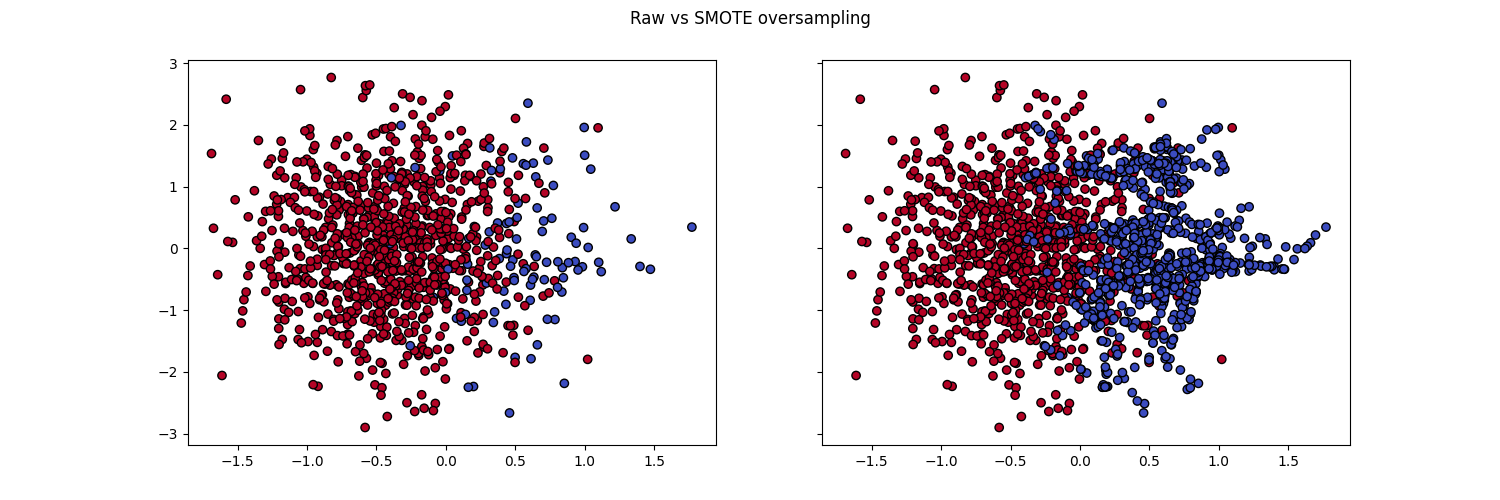
\includegraphics[width=0.8\textwidth]{images/Raw vs SMOTE oversampling.png}
    \caption{SMOTE örneği.}
    \label{fig:enter-label}
\end{figure}

\newpage

\subsection{ADASYN (Adaptive Synthetic Sampling)}
Azınlık sınıfındaki her örneğin etrafındaki hedeflenen komşuluk yoğunluğunu ölçer. Daha az temsil edilen örneklerin etrafında daha fazla sentetik örnek oluşturur. Bu azınlık sınıfındaki daha az temsil edilen bölgelerin daha fazla ağırlığı sahip olmasını sağlar. Sentetik örneklerin daha adaptif bir şekilde oluşturulması, daha az temsil edilen bölgelerde daha fazla vurgu yapılmasına olanak tanır.

\subsubsection{Çalışma Adımları}

\[ r_i = \frac{\text{KNN içindeki çoğunluk sınıfı komşularının sayısı}}{k} \]

Burada, $r_i$ azınlık sınıfına ait $x_i$ gözleminin zorluk derecesini temsil eder.

\[ G_i = r_i \times G \]

Burada, $G_i$ her bir azınlık sınıfı örneği için üretilecek sentetik veri miktarını, $r_i$ azınlık sınıfı örneğinin zorluk derecesini, $G$ toplamda üretilmesi gereken sentetik örnek sayısını temsil eder.

\[ \text{Yeni ornek} = x_i + \lambda \times (x_j - x_i) \]

Burada, $x_i$ azınlık sınıfına ait rastgele bir veri noktasını, $x_j$, $x_i$'nin en yakın komşularından birini, $\lambda$ 0 ile 1 arasında rastgele seçilen bir sayıyı temsil eder.

\begin{enumerate}
    \item İlk adımda, veri kümesindeki azınlık ve çoğunluk sınıfları belirlenir.
    \item ADASYN, her bir azınlık sınıfı gözlemi için çoğunluk sınıfına ait k-en yakın komşuları bulur.
    \item ADASYN, her bir azınlık sınıfı örneğinin zorluk derecesini hesaplar. Zorluk derecesi, bu azınlık örneğinin etrafındaki çoğunluk sınıfı örneklerinin sayısına bağlıdır. Eğer bir azınlık örneği çevresinde çoğunluk sınıfına ait çok fazla komşu varsa, bu örneğin sınıf sınırında olduğu ve sınıflandırılmasının daha zor olduğu anlamına gelir. Zorluk derecesi yüksek olan gözlemler, sınıf sınırında olup sınıflandırılması daha zor olan örneklerdir. ADASYN, bu örneklerin etrafında daha fazla sentetik veri üretmeye odaklanır.
    \item Azınlık sınıfına ait her bir veri noktası için zorluk derecelerini topladıktan sonra, her bir örnek için üretilecek sentetik veri miktarı hesaplar. Zorluk derecesi yüksek olan gözlemlere daha fazla sentetik örnek üretilirken, kolay sınıflandırılabilir gözlemler için daha az sentetik örnek üretilir.
    \item ADASYN, zorluk ağırlıklarına göre sentetik verileri üretir. Bu sentetik örnekler, azınlık sınıfındaki bir veri noktası ile onun en yakın komşuları arasındaki doğrusal interpolasyon kullanılarak üretilir.
\end{enumerate}

\subsubsection{Python Kod Implementasyonu}

\begin{lstlisting}[language=Python]
class ADASYN:
    def __init__(self, k_neighbors=3):
        self.k_neighbors = k_neighbors

    def fit_resample(self, X, y):
        class_counts = Counter(y)
        majority_class_count = max(class_counts.values())

        X_resampled = X
        y_resampled = y

        for class_label, count in class_counts.items():
            if count < majority_class_count:
                n_to_generate = majority_class_count - count
                X_class = X[y == class_label]

                nn = NearestNeighbors(n_neighbors=self.k_neighbors).fit(X_class)
                neighbors = nn.kneighbors(X_class, return_distance=False)

                synthetic_samples = np.zeros((n_to_generate, X.shape[1]))

                for i in range(n_to_generate):
                    sample_idx = np.random.randint(0, X_class.shape[0])
                    neighbor_idx = np.random.choice(neighbors[sample_idx][1:])

                    sample = X_class[sample_idx]
                    neighbor = X_class[neighbor_idx]

                    diff = neighbor - sample
                    gap = np.random.rand()
                    synthetic_samples[i] = sample + gap * diff

                X_resampled = np.vstack((X_resampled, synthetic_samples))
                y_resampled = np.hstack((y_resampled, np.full(n_to_generate, class_label)))

        return X_resampled, y_resampled
\end{lstlisting}

\newpage

\begin{figure}[h]
    \centering
    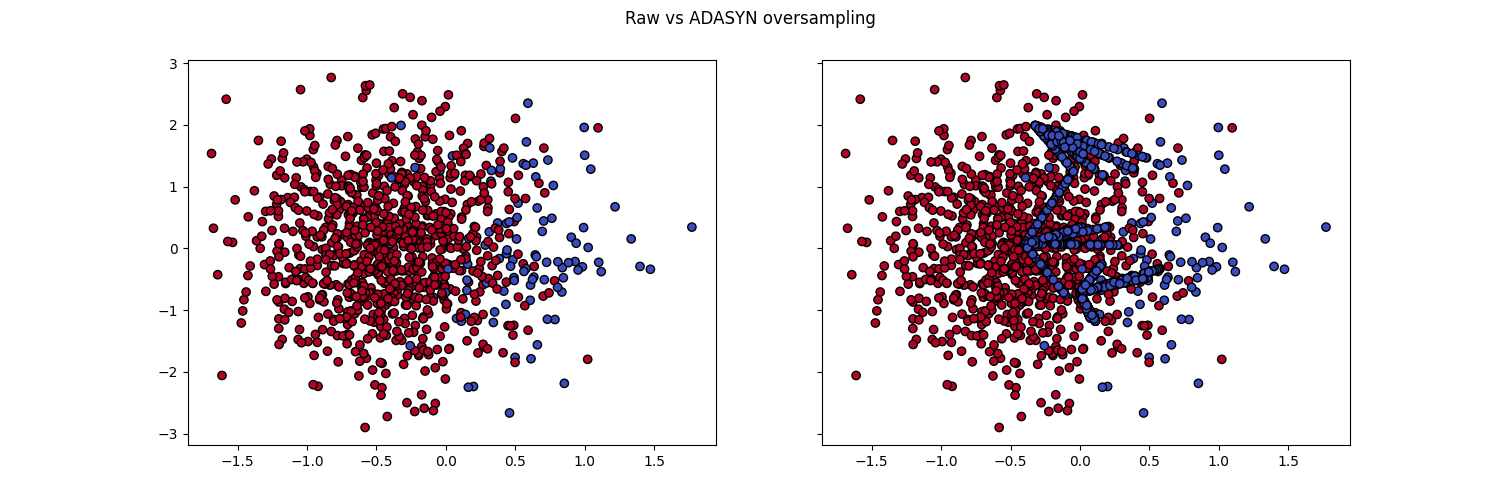
\includegraphics[width=1\textwidth]{images/Raw vs ADASYN oversampling.png}
    \caption{ADASYN örneği.}
    \label{fig:enter-label}
\end{figure}

\newpage

\subsection{Borderline-SMOTE}
Azınlık sınıfındaki örnekler arasında, sınıf sınırlarına yakın olanları belirler. Bu örnekler, genellikle çoğunluk sınıfına daha yakın olup karar sınırlarında yer alan veri noktalarıdır. Sınıf sınırındaki bu örnekler üzerinde sentetik örnekler oluşturarak azınlık sınıfının veri dağılımını artırır. Sentetik örnekler, gerçek verilere benzemesi için bu sınırlardaki veri noktalarının arasında oluşturulur.

\subsubsection{Çalışma Adımları}

\[ \text{Yeni ornek} = x_i + \lambda \times (x_j - x_i) \]

Burada, $x_i$ azınlık sınıfına ait rastgele bir veri noktasını, $x_j$, $x_i$'nin en yakın komşularından birini, $\lambda$ 0 ile 1 arasında rastgele seçilen bir sayıyı temsil eder.

\begin{enumerate}
    \item Öncelikle veri kümesindeki azınlık ve çoğunluk sınıfları belirlenir.
    \item Her bir azınlık sınıfı için k-en yakın komşular algoritması kullanılarak komşular belirlenir. Bu adım, azınlık sınıfı örneklerinin çoğunluk sınıfına ne kadar yakın olduğunu analiz etmek için kullanılır.
    \item Azınlık sınıfındaki her bir örneğin, çoğunluk sınıfı komşularıyla olan etkileşimi değerlendirilir ve bu örnekler üç gruba ayrılır:
    \begin{itemize}
        \item \textbf{Tehlikeli (Borderline) Örnekler}: Çoğunlukla çoğunluk sınıfı ile karışan ve sınıf sınırında bulunan azınlık sınıfı örnekleridir. Bu örnekler, sınıflandırma için kritik öneme sahiptir çünkü bu bölgede doğru bir sınıflandırma yapılmazsa model hatalı sınıflandırmalar yapabilir. Tehlikeli (borderline) örnekler, çoğunluk sınıfına yakın olduklarından dolayı modelin bu bölgedeki sınıf ayrımını güçlendirmek için sentetik veri üretiminin odak noktası olur.
        \item \textbf{Güvenli Örnekler}: Çoğunlukla diğer azınlık sınıfı komşularına sahip, sınıf sınırından uzakta olan güvenli örneklerdir.
        \item \textbf{Gürültü Örnekler}: Azınlık sınıfı olmasına rağmen çoğunluk sınıfı komşuları arasında izole olmuş ve çoğunluk sınıfına yakın yerlerde bulunan örneklerdir. Gürültü örnekler genellikle oversampling sürecine dahil edilmez.
    \end{itemize}
    \item Sadece sınıf sınırında, tehlikeli bölgede bulunan azınlık sınıfı örnekleri için sentetik veri üretimi yapılır. Borderline-SMOTE bu örneklerin en yakın azınlık sınıfı komşularıyla doğrusal interpolasyon yaparak sentetik veri üretir. Ancak, sadece sınıf sınırında bulunan tehlikeli örnekler üzerinden sentetik veri oluşturulur. Bu doğrusal interpolasyon yöntemi, sentetik verilerin, sınıf sınırlarında bulunan azınlık sınıfı örnekleri etrafında üretilmesini sağlar.
\end{enumerate}

\subsubsection{Python Kod Implementasyonu}

\begin{lstlisting}[language=Python]
class BorderlineSMOTE:
    def __init__(self, k_neighbors=5, m_neighbors=10):
        self.k_neighbors = k_neighbors
        self.m_neighbors = m_neighbors

    def fit_resample(self, X, y):
        classes, class_counts = np.unique(y, return_counts=True)
        majority_class = classes[np.argmax(class_counts)]
        minority_class = classes[np.argmin(class_counts)]

        minority_samples = X[y == minority_class]
        majority_samples = X[y == majority_class]

        n_minority_samples = minority_samples.shape[0]
        n_majority_samples = majority_samples.shape[0]
        n_to_generate = n_majority_samples - n_minority_samples

        if n_to_generate <= 0:
            return X, y

        nn_m = NearestNeighbors(n_neighbors=self.m_neighbors).fit(X)
        neighbors_m = nn_m.kneighbors(minority_samples, return_distance=False)

        danger_indices = []
        for i in range(n_minority_samples):
            majority_neighbors = sum(y[neighbors_m[i][1:]] == majority_class)
            if majority_neighbors > (self.m_neighbors / 2):
                danger_indices.append(i)
        
        danger_samples = minority_samples[danger_indices]
        if len(danger_samples) == 0:
            return X, y

        nn_k = NearestNeighbors(n_neighbors=self.k_neighbors).fit(minority_samples)
        neighbors_k = nn_k.kneighbors(danger_samples, return_distance=False)

        synthetic_samples = np.zeros((n_to_generate, X.shape[1]))

        for i in range(n_to_generate):
            sample_idx = np.random.randint(0, len(danger_samples))
            neighbor_idx = np.random.choice(neighbors_k[sample_idx][1:])
            
            sample = danger_samples[sample_idx]
            neighbor = minority_samples[neighbor_idx]
            
            diff = neighbor - sample
            gap = np.random.rand()
            synthetic_samples[i] = sample + gap * diff

        X_resampled = np.vstack((X, synthetic_samples))
        y_resampled = np.hstack((y, np.full(n_to_generate, minority_class)))
        return X_resampled, y_resampled
\end{lstlisting}

\begin{figure}[h]
    \centering
    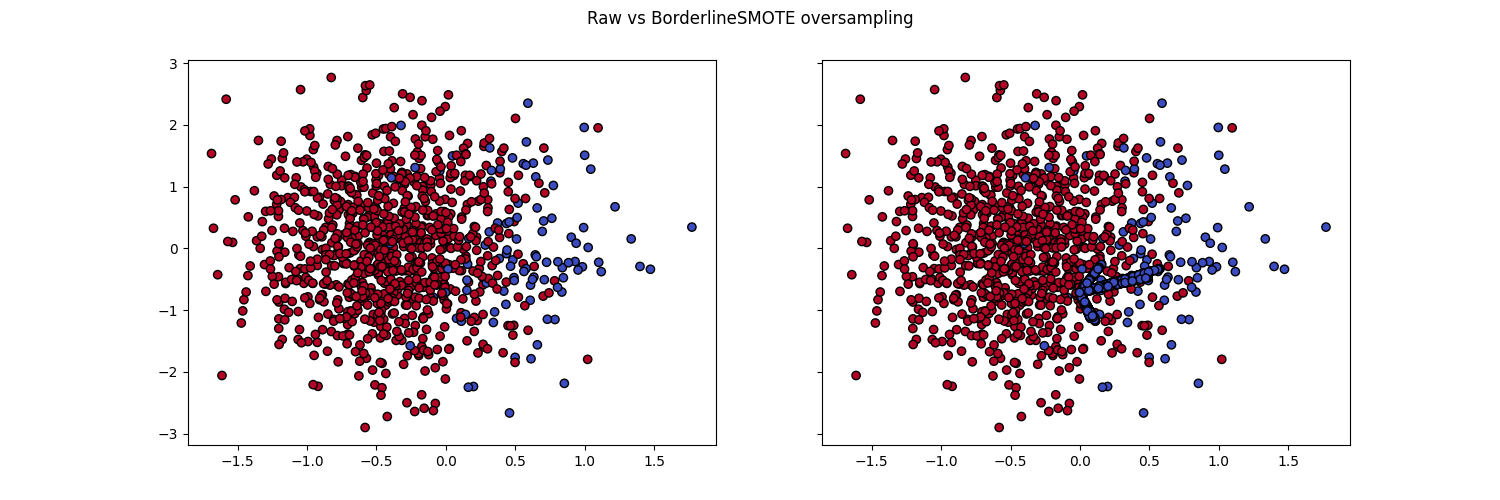
\includegraphics[width=1\textwidth]{images/Raw vs BorderlineSMOTE oversampling.png}
    \caption{Borderline-SMOTE örneği.}
    \label{fig:enter-label}
\end{figure}

\newpage

\subsection{Random Over Sampling}
Azınlık sınıfındaki örneklerin sayısına eşit olacak şekilde, çoğunluk sınıfındaki örnekler rastgele seçilerek artırılır. Bu seçilen örnekler, azınlık sınıfındaki mevcut örneklerle birleştirilerek dengeli bir veri seti oluşturulur. Mevcut veri setini değiştirmez sadece örneklerin tekrarlanmasını kullanır.

\subsubsection{Çalışma Adımları}

\begin{enumerate}
    \item Veri setindeki sınıf dengesizliğini anlamak için önce azınlık ve çoğunluk sınıfları belirlenir.
    \item Çoğunluk sınıfının veri kümesinde kaç gözleme sahip olduğu tespit edilir. Bu adım, azınlık sınıfına ne kadar fazla sentetik örnek ekleneceğini belirler. RandomOverSampler, azınlık sınıfının gözlem sayısını çoğunluk sınıfının gözlem sayısına eşitlemeye çalışır.
    \item Azınlık sınıfı gözlemlerinden rastgele seçim yapılır. RandomOverSampler, azınlık sınıfından rastgele gözlemleri tekrar tekrar seçerek çoğunluk sınıfıyla aynı sayıda gözlem elde edinceye kadar süreci devam ettirir. Seçilen gözlemler mevcut veri setindeki gözlemlerin birebir kopyasıdır; yeni veri noktaları oluşturulmaz, sadece mevcut örnekler çoğaltılır. Bu aşamada rastgele seçim tamamen olasılıksaldır, yani örnekler veri kümesindeki herhangi bir örnekten bağımsız olarak eşit olasılıkla seçilir.
    \item Rastgele seçilen azınlık sınıfı gözlemleri veri setine eklenir. Bu, çoğunluk sınıfının boyutuna kadar devam eder. Her seçilen gözlem, veri setine bir kopyası olarak eklenir, böylece azınlık sınıfının boyutu, çoğunluk sınıfıyla eşit hale gelir.
\end{enumerate}

\subsubsection{Python Kod Implementasyonu}

\begin{lstlisting}[language=Python]
class RandomOverSampler:
    def __init__(self):
        pass

    def fit_resample(self, X, y):
        class_counts = Counter(y)
        max_class_count = max(class_counts.values())

        X_resampled = []
        y_resampled = []

        for class_label, count in class_counts.items():
            X_class = X[y == class_label]

            if count < max_class_count:
                n_to_generate = max_class_count - count
                random_indices = np.random.randint(0, X_class.shape[0], size=n_to_generate)
                X_oversampled = X_class[random_indices]
                X_resampled.append(np.vstack((X_class, X_oversampled)))
                y_resampled.append(np.hstack((np.full(count, class_label), 
                                              np.full(n_to_generate, class_label))))
            else:
                X_resampled.append(X_class)
                y_resampled.append(np.full(X_class.shape[0], class_label))

        X_resampled = np.vstack(X_resampled)
        y_resampled = np.hstack(y_resampled)
        return X_resampled, y_resampled
\end{lstlisting}

\begin{figure}[h]
    \centering
    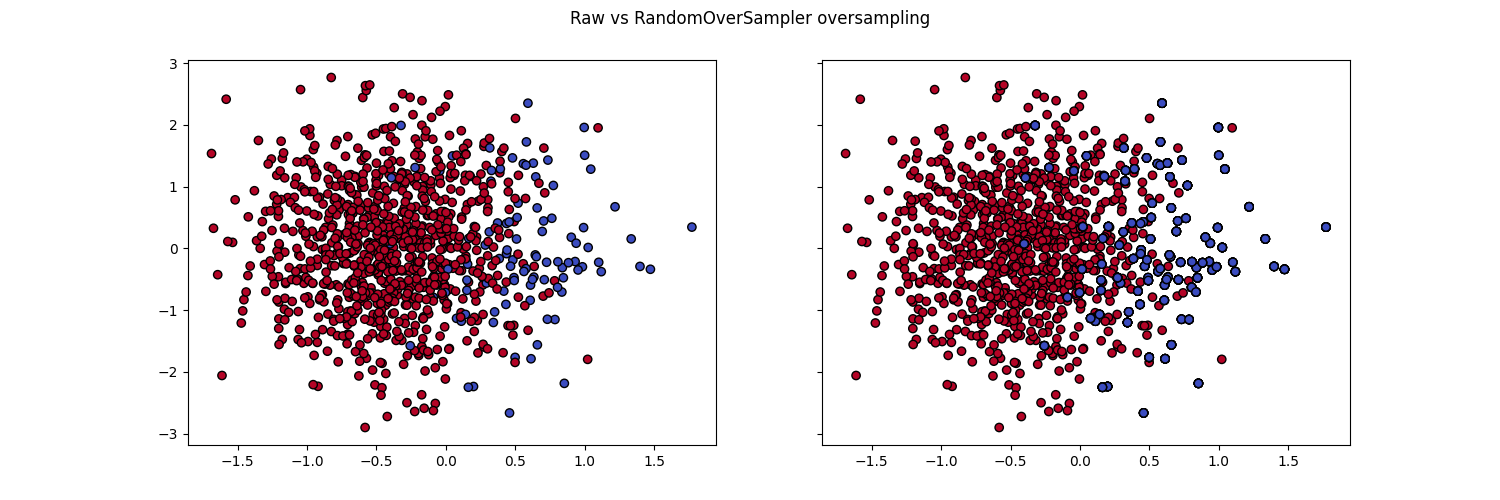
\includegraphics[width=1\textwidth]{images/Raw vs RandomOverSampler oversampling.png}
    \caption{RandomOverSampler örneği.}
    \label{fig:enter-label}
\end{figure}

\newpage

\subsection{Cluster Centroids}
Azınlık sınıfındaki veri noktalarının küme merkezlerini hesaplar. Bu küme merkezleri, çoğunluk sınıfındaki veri noktalarıyla değiştirilir. Bu, azınlık sınıfını temsil etmek için yeni bir alt örneklem oluşturur.

\subsubsection{Çalışma Adımları}

\begin{enumerate}
    \item Veri setindeki sınıf dağılımı incelenir ve azınlık ve çoğunluk sınıfları belirlenir.
    \item ClusterCentroids yönteminin temelinde, çoğunluk sınıfındaki gözlemlerin merkezlerini (centroid) bulmak için k-means kümeleme algoritması kullanılır. K-means, veri kümesini k adet kümeye ayırarak her küme için bir merkez belirler. ClusterCentroids, bu merkez noktalarını seçerek çoğunluk sınıfını azaltır. Bu aşamada, çoğunluk sınıfındaki gözlemler birkaç küme (cluster) oluşturacak şekilde gruplanır ve her küme için bir centroid (merkez noktası) hesaplanır. Bu centroid, küme içindeki tüm gözlemlerin ortalama pozisyonunu temsil eder. K-means algoritması, kümeleri oluştururken her gözlemi en yakın merkeze atar ve bu şekilde kümeleri optimize eder.
    \item K-means algoritması tarafından çoğunluk sınıfındaki gözlemler için oluşturulan her bir kümenin merkezi (centroid), çoğunluk sınıfını temsil eden yeni gözlem olarak seçilir. Bu merkez noktaları, her kümenin genelleştirilmiş bir özetidir ve çoğunluk sınıfındaki gözlemleri daha dengeli ve temsili bir şekilde azaltır. Bu merkezler, çoğunluk sınıfının veri setindeki genel dağılımını en iyi şekilde temsil etmeyi hedefler. Seçilen bu centroidler, çoğunluk sınıfının sayısını düşürerek azınlık sınıfıyla dengelenmesini sağlar.
    \item Centroidler belirlendikten sonra, veri setindeki çoğunluk sınıfı gözlemleri bu merkezlerle değiştirilir. Yani çoğunluk sınıfındaki orijinal gözlemler veri setinden çıkarılır ve yerlerine bu merkezler eklenir. Bu sayede çoğunluk sınıfının sayısı azaltılarak azınlık sınıfı ile dengelenir.
\end{enumerate}

\subsubsection{Python Kod Implementasyonu}

\begin{lstlisting}[language=Python]
class ClusterCentroids:
    def __init__(self, n_clusters=None):
        self.n_clusters = n_clusters

    def fit_resample(self, X, y):
        class_counts = Counter(y)
        minority_class_count = min(class_counts.values())

        X_resampled = []
        y_resampled = []

        for class_label, count in class_counts.items():
            X_class = X[y == class_label]

            if count > minority_class_count:
                kmeans = KMeans(n_clusters=minority_class_count)
                kmeans.fit(X_class)
                centroids = kmeans.cluster_centers_
                X_resampled.append(centroids)
                y_resampled.append(np.full(minority_class_count, class_label))
            else:
                X_resampled.append(X_class)
                y_resampled.append(np.full(X_class.shape[0], class_label))

        X_resampled = np.vstack(X_resampled)
        y_resampled = np.hstack(y_resampled)
        return X_resampled, y_resampled
\end{lstlisting}

\begin{figure}[h]
    \centering
    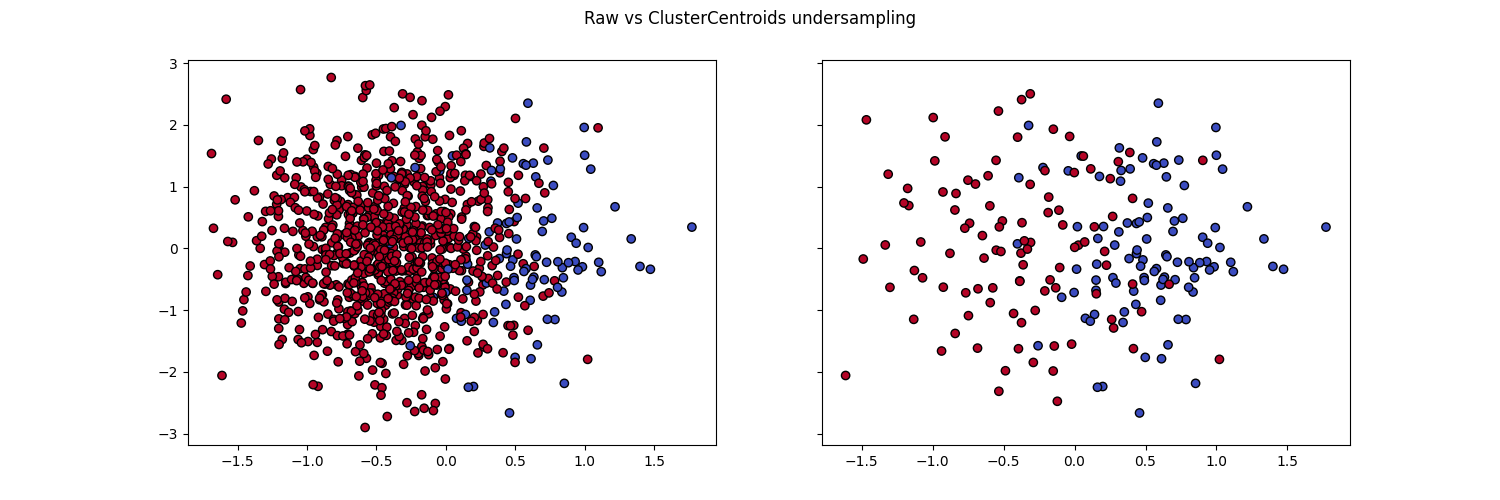
\includegraphics[width=1\textwidth]{images/Raw vs ClusterCentroids undersampling.png}
    \caption{ClusterCentroids örneği.}
    \label{fig:enter-label}
\end{figure}

\newpage

\subsection{Random Under Sampling}
Çoğunluk sınıfından rastgele örnekler seçerek, azınlık sınıfındaki örnek sayısıyla aynı sayıya düşürür. Bu seçilen örnekler, çoğunluk sınıfındaki veri sayısını azaltarak daha dengeli bir veri seti oluşturur.

\subsubsection{Çalışma Adımları}

\begin{enumerate}
    \item İlk adımda, veri setindeki her sınıfın gözlem sayıları hesaplanır ve hangi sınıfın azınlık (minority), hangi sınıfın çoğunluk (majority) sınıf olduğu belirlenir.
    \item RandomUnderSampler, çoğunluk sınıfındaki gözlemlerden rastgele örnekler seçer. Bu rastgele seçilen örnekler, veri setinden çıkarılarak çoğunluk sınıfının boyutunu azaltır. Burada dikkat edilmesi gereken nokta, azınlık sınıfına dokunulmaması ve yalnızca çoğunluk sınıfındaki gözlemlerin azaltılmasıdır.
    \item RandomUnderSampler yönteminde, veri bilimci çoğunluk ve azınlık sınıflarının nasıl dengeleneceğine karar verebilir. Bu dengeleme, "sampling\_strategy" adı verilen bir parametre ile kontrol edilir. Eğer "sampling\_strategy" parametresi belirtilmezse, varsayılan olarak çoğunluk sınıfı azınlık sınıfıyla eşitlenir. Bu parametre ile aşağıdaki senaryolardan biri seçilebilir:
    \begin{itemize}
        \item \textbf{Azınlık sınıfına eşitleme}: Çoğunluk sınıfı, azınlık sınıfıyla aynı sayıya indirgenir. Bu, en yaygın kullanılan stratejidir ve sınıf dengesizliğini tamamen giderir.
        \item \textbf{Belirli bir oran}: Çoğunluk sınıfını, azınlık sınıfından daha büyük ama belirli bir oranla daha küçük hale getirmek mümkündür. Örneğin, çoğunluk sınıfının azınlık sınıfının iki katı kadar olmasını sağlayabilirsiniz.
    \end{itemize}
\end{enumerate}

\subsubsection{Python Kod Implementasyonu}

\begin{lstlisting}[language=Python]
class RandomUnderSampler:
    def __init__(self):
        pass

    def fit_resample(self, X, y):
        classes, class_counts = np.unique(y, return_counts=True)

        min_class_size = np.min(class_counts)

        X_resampled = []
        y_resampled = []

        for class_label in classes:
            class_samples = X[y == class_label]
            n_class_samples = class_samples.shape[0]

            if n_class_samples > min_class_size:
                selected_indices = np.random.choice(class_samples.shape[0], 
                                                    min_class_size, replace=False)
                selected_samples_resampled = class_samples[selected_indices]
            else:
                selected_samples_resampled = class_samples
            
            X_resampled.append(selected_samples_resampled)
            y_resampled.append(np.full(min_class_size, class_label))
            
        X_resampled = np.vstack(X_resampled)
        y_resampled = np.hstack(y_resampled)
        return X_resampled, y_resampled
\end{lstlisting}

\begin{figure}[h]
    \centering
    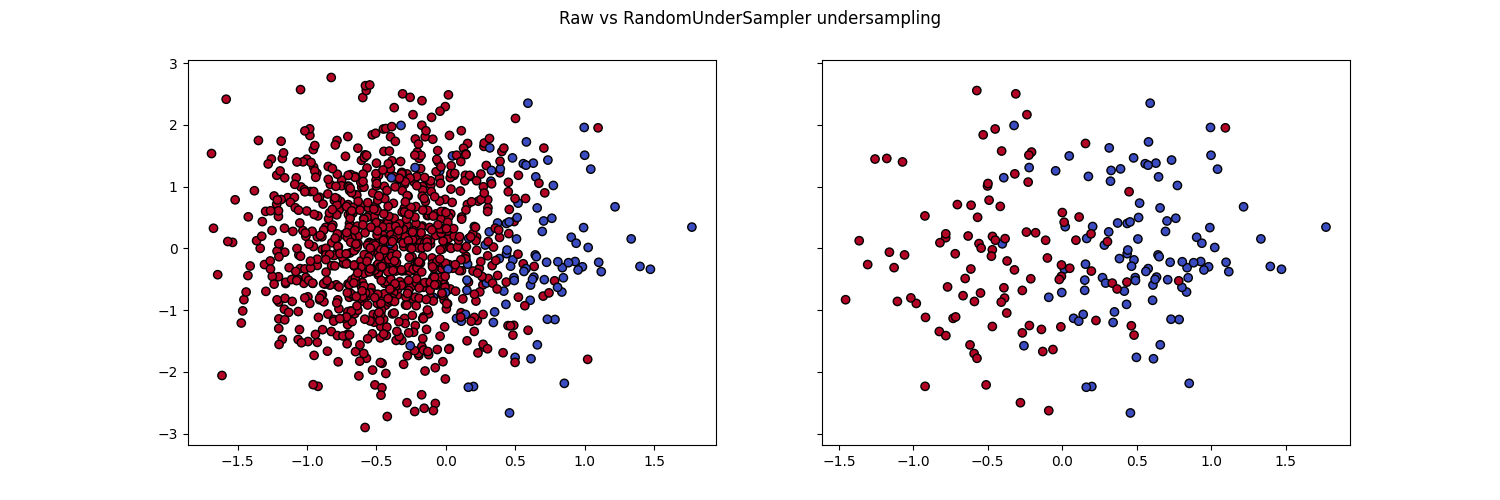
\includegraphics[width=1\textwidth]{images/Raw vs RandomUnderSampler undersampling.png}
    \caption{RandomUnderSampler örneği.}
    \label{fig:enter-label}
\end{figure}

\newpage

\subsection{Near Miss}
Azınlık sınıfına daha yakın olan çoğunluk sınıfı örneklerini belirlemek için bir kriter kullanır. Bu kriter, belirli bir eşik değeri veya uzaklık ölçüsüne dayanır. Seçilen çoğunluk sınıfı örnekleri, azınlık sınıfı ile aralarındaki uzaklık veya farklılık kriterini en iyi şekilde karşılayan örneklerdir. Bu örnekler seçilerek alt örnekleme işlemi gerçekleştirilir.

\subsubsection{Çalışma Adımları}

\begin{enumerate}
    \item İlk adım olarak, veri setinde hangi sınıfın azınlık (minority) ve hangi sınıfın çoğunluk (majority) olduğuna karar verilir.
    \item NearMiss yöntemi, gözlemler arasındaki mesafeleri kullanarak çoğunluk sınıfından seçilecek örnekleri belirler.
    \item NearMiss yönteminin üç farklı versiyonu vardır: NearMiss-1, NearMiss-2, ve NearMiss-3. Bu üç yaklaşım da farklı stratejilerle çoğunluk sınıfından örnek seçimi yapar. Her biri, azınlık sınıfı etrafındaki çoğunluk sınıfı gözlemlerini seçerek, sınıf sınırlarını daha net hale getirmeye çalışır.
    \begin{itemize}
        \item \textbf{NearMiss-1}: Azınlık sınıfındaki her bir gözlem için, ona en yakın olan belirli sayıda çoğunluk sınıfı gözlemini seçer. Yani, azınlık sınıfındaki her gözleme en yakın çoğunluk sınıfı gözlemleri belirlenir ve sadece bu gözlemler veri setinde tutulur. Azınlık sınıfındaki her örnek için çoğunluk sınıfındaki gözlemlerle olan mesafeler hesaplanır. En küçük mesafeye sahip k tane çoğunluk sınıfı gözlemi seçilir. Seçilen çoğunluk sınıfı örnekleri korunur, diğerleri çıkarılır.
        \item \textbf{NearMiss-2}: Her bir çoğunluk sınıfı gözlemi, en uzak azınlık sınıfı gözlemlerine göre seçilir. Bu sayede, çoğunluk sınıfındaki gözlemler arasındaki çeşitlilik artar. Çoğunluk sınıfındaki her örnek için, azınlık sınıfı gözlemleriyle olan mesafeler hesaplanır. Çoğunluk sınıfı gözlemleri arasından, azınlık sınıfına en uzak olan k tane çoğunluk sınıfı gözlemi seçilir ve veri setinde tutulur. Diğer çoğunluk sınıfı gözlemleri çıkarılır.
        \item \textbf{NearMiss-3}: NearMiss-1 ve NearMiss-2'nin bir kombinasyonudur. Bu yöntem, her azınlık sınıfı gözlemi için en yakın çoğunluk sınıfı gözlemlerini seçmek yerine, her çoğunluk sınıfı gözlemi için en yakın azınlık sınıfı gözlemlerini kullanır. Böylece her çoğunluk sınıfı örneği, en yakın azınlık sınıfı gözlemleriyle temsil edilir. Çoğunluk sınıfındaki her gözlem için, en yakın k tane azınlık sınıfı gözlemi belirlenir. Çoğunluk sınıfından en yakın azınlık sınıfına sahip gözlemler veri setinde tutulur. Diğer çoğunluk sınıfı gözlemleri çıkarılır.
    \end{itemize}
    \item NearMiss algoritmasının varyasyonlarından birinin uygulanması sonucunda, veri setinde azınlık ve çoğunluk sınıflarındaki gözlem sayıları daha dengeli hale getirilir
\end{enumerate}

\subsubsection{Python Kod Implementasyonu}

\begin{lstlisting}[language=Python]
class NearMiss:
    def __init__(self, n_neighbors=3):
        self.n_neighbors = n_neighbors

    def fit_resample(self, X, y):
        classes, class_counts = np.unique(y, return_counts=True)
        
        min_class_size = np.min(class_counts)
        
        X_resampled = []
        y_resampled = []
        
        for class_label in classes:
            class_samples = X[y == class_label]
            n_class_samples = class_samples.shape[0]
            
            if n_class_samples > min_class_size:
                nn = NearestNeighbors(n_neighbors=self.n_neighbors)
                nn.fit(class_samples)
                
                distances, _ = nn.kneighbors(class_samples)
                
                sorted_idx = np.argsort(distances.mean(axis=1))
                
                selected_samples = class_samples[sorted_idx[:min_class_size]]
            else:
                selected_samples = class_samples
            
            X_resampled.append(selected_samples)
            y_resampled.append(np.full(min_class_size, class_label))
        
        X_resampled = np.vstack(X_resampled)
        y_resampled = np.hstack(y_resampled)
        return X_resampled, y_resampled
\end{lstlisting}

\newpage

\begin{figure}[h]
    \centering
    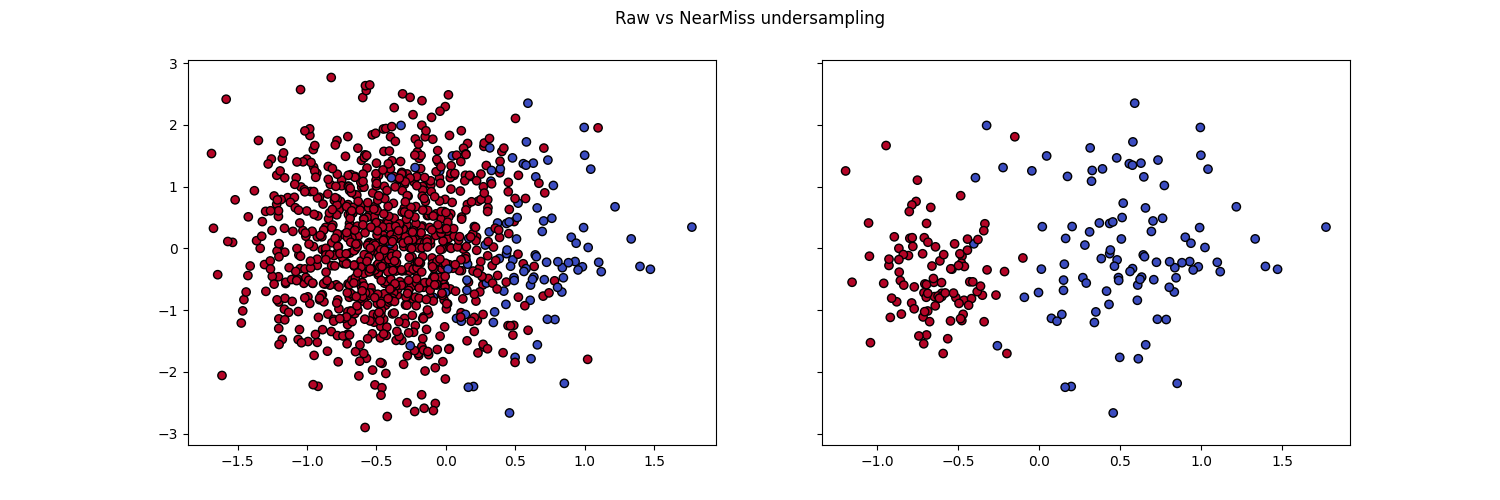
\includegraphics[width=0.8\textwidth]{images/Raw vs NearMiss undersampling.png}
    \caption{NearMiss örneği.}
    \label{fig:enter-label}
\end{figure}

\newpage

\subsection{Tomek Links}
Veri setindeki her bir veri noktası için o veri noktasına en yakın komşusunu bulur. Eğer iki veri noktası birbirlerinin en yakın komşusuysa ve aynı sınıfa ait değillerse, bu iki veri noktası arasındaki ilişkiyi (tomek link) belirler. Bu tomek linke sahip olan veri noktalarından çoğunluk sınıfına ait olan çıkararak veri dengesizliğini azaltır.

\subsubsection{Çalışma Adımları}

\begin{enumerate}
    \item İlk adım olarak, veri setinde hangi sınıfın azınlık (minority) ve hangi sınıfın çoğunluk (majority) olduğuna bakılır.
    \item Tomek Links’in merkezinde, iki farklı sınıfa ait gözlemlerden oluşan komşu çiftlerinin tespiti vardır. Tomek Links algoritması şu adımları izler:
    \begin{itemize}
        \item Tüm veri setindeki örnekler arasında mesafe hesaplanır. Genellikle Euclidean mesafesi kullanılır. Mesafe hesaplandıktan sonra, her örneğin en yakın komşusu bulunur.
        \item Eğer bir örneğin en yakın komşusu, farklı bir sınıfa aitse bu iki örnek bir Tomek Link çifti olarak tanımlanır. Bu durumda, azınlık sınıfına ait bir örneğin en yakın komşusu çoğunluk sınıfına ait olmalıdır ve bu iki örnek birbirine çok yakın mesafede olmalıdır.
        \item Tomek Link çiftleri, genellikle sınıf sınırlarında bulunur. Bu sınırlar, modelin hangi sınıfa ait olduğunu öğrenmekte zorlandığı yerlerdir. Bu nedenle, Tomek Links bu sınırları temizleyerek sınıflar arasındaki farkı daha net hale getirmeyi amaçlar.
    \end{itemize}
    \item Tomek Link çiftleri belirlendikten sonra, çoğunluk sınıfına ait gözlemler bu çiftlerden çıkarılır. Bunun nedeni, bu gözlemlerin sınıf sınırlarında yer alarak modelin öğrenme sürecinde karışıklık yaratmasıdır. Tomek Links, yalnızca çoğunluk sınıfına ait olan gözlemleri kaldırarak azınlık sınıfı örneklerine dokunmaz. Böylece, veri setindeki azınlık sınıfının korunması sağlanır.
\end{enumerate}

\subsubsection{Python Kod Implementasyonu}

\begin{lstlisting}[language=Python]
class TomekLinks:
    def __init__(self):
        pass

    def fit_resample(self, X, y):
        nn = NearestNeighbors(n_neighbors=2)
        nn.fit(X)
        
        distances, indices = nn.kneighbors(X)
        
        tomek_links = []
        
        for i in range(len(X)):
            neighbor_idx = indices[i][1]
            
            if y[i] != y[neighbor_idx]:
                tomek_links.append((i, neighbor_idx))
        
        indices_to_remove = set()
        for i, j in tomek_links:
            if y[i] > y[j]:
                indices_to_remove.add(i)
            else:
                indices_to_remove.add(j)
        
        mask = np.ones(len(X), dtype=bool)
        mask[list(indices_to_remove)] = False
        
        X_resampled = X[mask]
        y_resampled = y[mask]

        class_counts = Counter(y_resampled)
        min_class_count = min(class_counts.values())

        X_balanced = []
        y_balanced = []

        for class_label in class_counts.keys():
            class_indices = np.where(y == class_label)[0]
            selected_indices = np.random.choice(class_indices, 
                                                min_class_count, 
                                                replace=False)
            X_balanced.append(X[selected_indices])
            y_balanced.append(y[selected_indices])

        X_balanced = np.vstack(X_balanced)
        y_balanced = np.hstack(y_balanced)
        
        return X_balanced, y_balanced
\end{lstlisting}

\newpage

\begin{figure}[h]
    \centering
    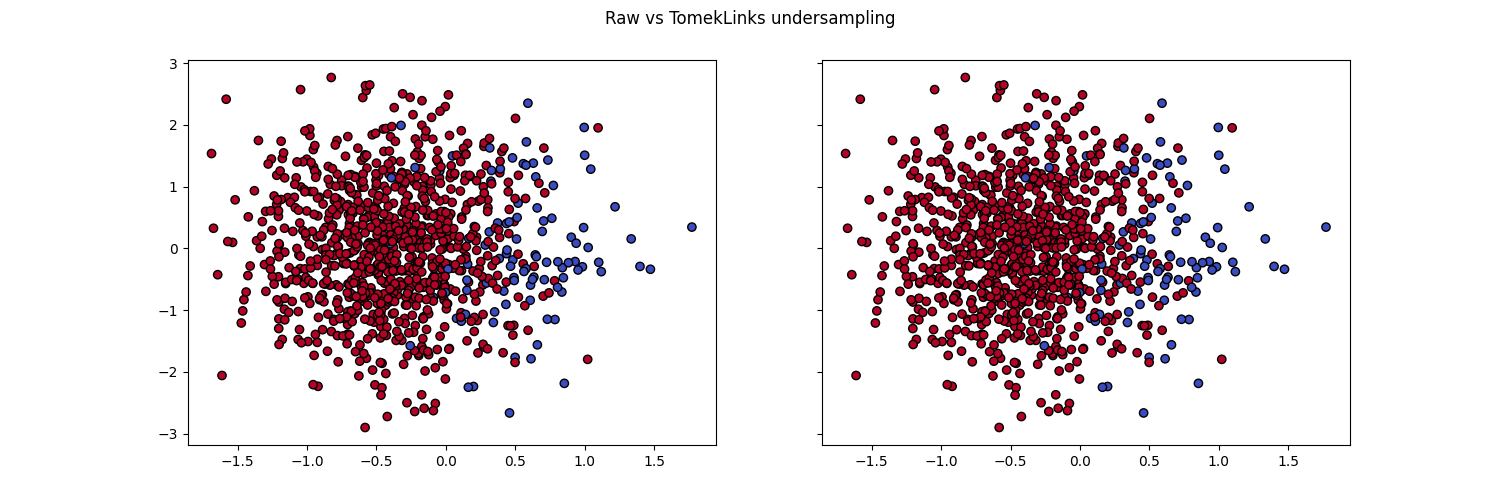
\includegraphics[width=0.8\textwidth]{images/Raw vs TomekLinks undersampling.png}
    \caption{TomekLinks örneği.}
    \label{fig:enter-label}
\end{figure}

\newpage

\subsection{Condensed Nearest Neighbour}
Veri setindeki bir örnek seçilir. Seçilen bu örnek aynı sınıfa ait komşuları ile karşılaştırılır. Eğer bu örnek, aynı sınıfa ait komşularından farklı bir sınıfa aitse, bu örnek korunur ve yeni alt örnekleme setine eklenir. Diğer tüm örnekler bu kriterlere göre kontrol edilir ve veri setinden aynı bilgiyi koruyarak daha küçük bir alt örnekleme seti oluşturulur.

\subsubsection{Çalışma Adımları}

\begin{enumerate}
    \item İlk olarak veri setini iki sınıfa ayırır: azınlık ve çoğunluk sınıfı.
    \item CNN algoritması, azınlık sınıfı gözlemlerinin tamamını ve çoğunluk sınıfından rastgele seçilen bir veya birkaç örneği alarak bir başlangıç kümesi oluşturur. Bu küme, daha sonra büyütülerek çoğunluk sınıfındaki diğer örnekleri temsil edecek şekilde genişletilir.
    \item Başlangıç kümesi oluşturulduktan sonra, kalan çoğunluk sınıfı gözlemleri, başlangıç kümesine eklenip eklenmeyeceğine karar vermek için en yakın komşu (nearest neighbor) sınıflandırmasına tabi tutulur. 
    \begin{itemize}
        \item Kalan çoğunluk sınıfındaki her bir gözlem için, başlangıç kümesindeki gözlemlere olan mesafeler hesaplanır. 
        \item Eğer çoğunluk sınıfındaki bir gözlem, başlangıç kümesine yanlış sınıflandırılmışsa (yani, yanlış sınıf ile tahmin edilmişse), bu gözlem başlangıç kümesine eklenir. 
        \item Eğer çoğunluk sınıfındaki gözlem doğru sınıflandırılmışsa, bu gözlem veri setinden çıkarılır ve alt örnekleme yapılmış veri setine dahil edilmez.
    \end{itemize}
    \item Başlangıç kümesine, yanlış sınıflandırılan çoğunluk sınıfı gözlemleri eklendikçe, bu küme genişler. Hedef, sınıf sınırlarını doğru bir şekilde temsil edebilen bir veri kümesi oluşturmaktır. Bu süreç, tüm gözlemler doğru sınıflanana kadar devam eder. Her iterasyonda, doğru sınıflandırılamayan yeni çoğunluk sınıfı örnekleri kümeye eklenir. Küme genişledikçe, daha az sayıda gözlem eklenmeye başlar çünkü çoğu örnek doğru sınıflandırılır hale gelir. Sonunda, gereksiz gözlemler çıkarılmış olur ve daha küçük bir eğitim veri kümesi elde edilir.
    \item CNN algoritması, tüm çoğunluk sınıfı gözlemleri doğru sınıflandırılana kadar iterasyonlarla devam eder. Bu noktada, eklemeye gerek duyulan yeni gözlem kalmaz ve algoritma durur. Elde edilen alt küme, veri setinin daha kompakt ve daha dengeli bir temsilidir. Algoritma, tüm gözlemler doğru sınıflandırıldığında durur. Alt küme, azınlık sınıfı örnekleri ve doğru sınıflandırılamayan çoğunluk sınıfı örneklerinden oluşur.
\end{enumerate}

\subsubsection{Python Kod Implementasyonu}

\begin{lstlisting}[language=Python]
class CondensedNearestNeighbors:
    def __init__(self, k_neighbors=1):
        self.k_neighbors = k_neighbors

    def fit_resample(self, X, y):
        class_counts = Counter(y)
        min_class_size = min(class_counts.values())
        classes = np.unique(y)

        X_resampled = []
        y_resampled = []

        for class_label in classes:
            X_class = X[y == class_label]
            y_class = y[y == class_label]

            idx_selected = [0]
            knn = KNeighborsClassifier(n_neighbors=self.k_neighbors)

            while len(idx_selected) < min_class_size:
                X_selected = X_class[idx_selected]
                y_selected = y_class[idx_selected]

                knn.fit(X_selected, y_selected)

                for i in range(len(X_class)):
                    if i not in idx_selected:
                        y_pred = knn.predict([X_class[i]])
                        if y_pred != y_class[i]:
                            idx_selected.append(i)

                if len(idx_selected) > min_class_size:
                    idx_selected = np.random.choice(idx_selected, 
                                                    min_class_size,
                                                    replace=False)

            X_resampled.append(X_class[idx_selected])
            y_resampled.append(y_class[idx_selected])

        X_resampled = np.vstack(X_resampled)
        y_resampled = np.hstack(y_resampled)
        return X_resampled, y_resampled
\end{lstlisting}

\newpage

\begin{figure}[h]
    \centering
    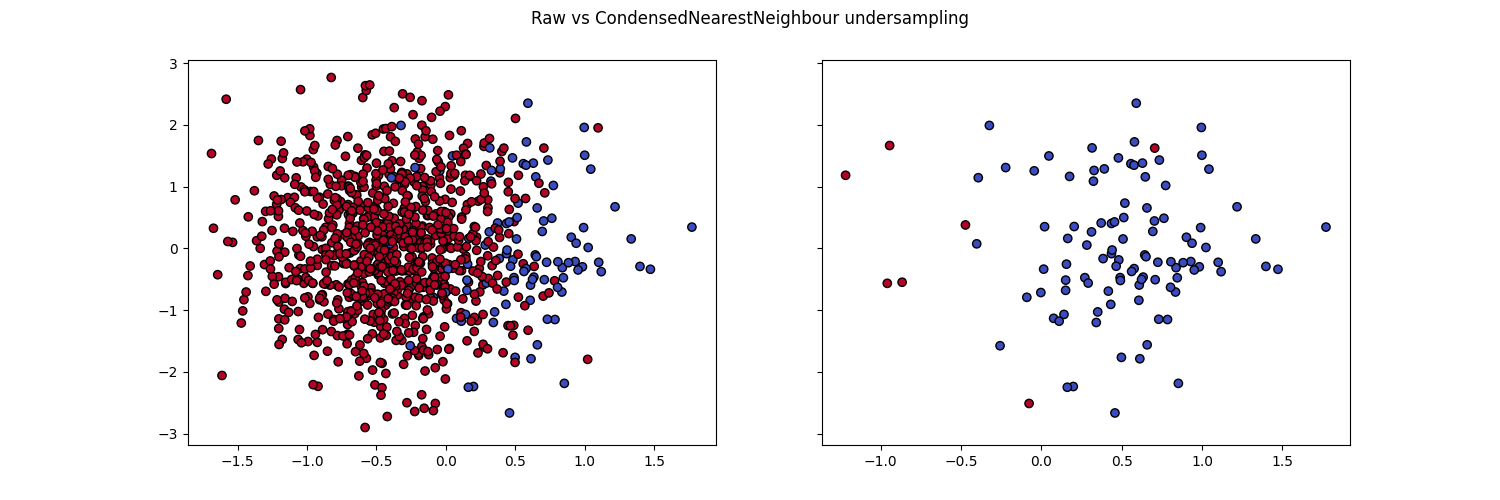
\includegraphics[width=0.8\textwidth]{images/Raw vs CondensedNearestNeighbour undersampling.png}
    \caption{CondensedNearestNeighbour örneği.}
    \label{fig:enter-label}
\end{figure}

\newpage

\subsection{One Sided Selection}
Azınlık sınıfından rastgele bir örnek seçilir. Seçilen bu örnek, çoğunluk sınıfındaki komşuları ile karşılaştırılır. Eğer bu örnek, çoğunluk sınıfındaki örneklerin etkileşimli olduğu bir bölgede bulunmuyorsa ve azınlık sınıfına aitse, bu örnek korunur ve yeni alt örnekleme setine eklenir. Diğer azınlık sınıfı örnekleri de bu şekilde kontrol edilir ve belirli bir kriteri sağlayan örnekler korunarak daha dengeli bir alt örnekleme seti oluşturulur.

\subsubsection{Çalışma Adımları}

\begin{enumerate}
    \item Öncelikle veri seti çoğunluk ve azınlık sınıfı gözlemlerine ayrılır.
    \item Veri setindeki tüm azınlık sınıfı örnekleri başlangıç kümesine eklenir. Çoğunluk sınıfı örnekleri OSS algoritması ile incelenmeye başlanır.
    \item İlk adımda, veri setindeki gürültülü ve yanlış sınıflandırılabilecek çoğunluk sınıfı örnekleri belirlenir ve veri setinden çıkarılır. Bunun için k-en yakın komşu (k-NN) algoritması kullanılır. Çoğunluk sınıfındaki örnekler, k-NN ile tekrar tekrar sınıflandırılır ve yanlış sınıflandırılanlar gürültü olarak kabul edilip kaldırılır.
    \item Gürültü temizlendikten sonra, Tomek Links yöntemi kullanılarak sınırda yer alan gözlemler temizlenir. Tomek Links, iki farklı sınıfa ait örneklerin birbirine en yakın komşular olduğu çiftlerdir. Bu gözlemler sınırda yer aldıkları için, sınıflandırmayı zorlaştırabilir. OSS, bu çiftleri bulur ve çoğunluk sınıfındaki gözlemleri temizler.
    \item Noise Removal ve Tomek Links adımlarından sonra, veri setindeki gereksiz veya yanlış sınıflandırılabilir çoğunluk sınıfı örnekleri kaldırılmış olur. Sonuçta, daha küçük ve daha dengeli bir veri seti elde edilir.
\end{enumerate}

\subsubsection{Python Kod Implementasyonu}

\begin{lstlisting}[language=Python]
class OneSidedSelection:
    def __init__(self, k_neighbors=1):
        self.k_neighbors = k_neighbors

    def fit_resample(self, X, y):
        class_counts = Counter(y)
        minority_class = min(class_counts, key=class_counts.get)
        minority_class_size = class_counts[minority_class]

        X_resampled = []
        y_resampled = []

        for class_label, count in class_counts.items():
            X_class = X[y == class_label]

            if class_label != minority_class:
                knn = KNeighborsClassifier(n_neighbors=self.k_neighbors)
                knn.fit(X_class, np.full(X_class.shape[0], class_label))

                selected_samples = []
                for sample in X_class:
                    neighbors = knn.kneighbors([sample], 
                                        return_distance=False).flatten()
                    if np.all(y[neighbors] == class_label):
                        selected_samples.append(sample)

                selected_samples = np.array(selected_samples)
                if len(selected_samples) > minority_class_size:
                    selected_samples = selected_samples[
                        np.random.choice(len(selected_samples), 
                        minority_class_size, 
                        replace=False)]

                X_resampled.append(selected_samples)
                y_resampled.append(np.full(minority_class_size, class_label))
            else:
                X_resampled.append(X_class)
                y_resampled.append(np.full(X_class.shape[0], class_label))

        X_resampled = np.vstack(X_resampled)
        y_resampled = np.hstack(y_resampled)

        return X_resampled, y_resampled
\end{lstlisting}

\begin{figure}[h]
    \centering
    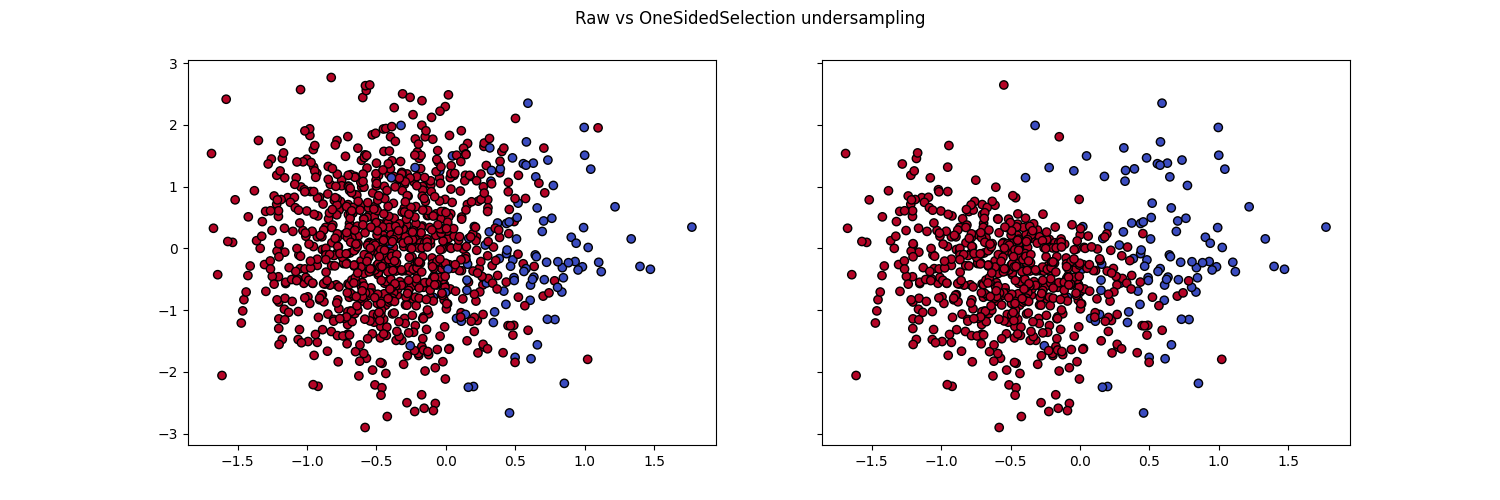
\includegraphics[width=0.8\textwidth]{images/Raw vs OneSidedSelection undersampling.png}
    \caption{OneSidedSelection örneği.}
    \label{fig:enter-label}
\end{figure}

\newpage

\subsection{Neighbourhood Cleaning Rule}
Azınlık sınıfındaki bir örnek seçilir. Seçilen bu örnek, çoğunluk ve azınlık sınıflarının sınırlarındaki bölgelerdeki örnekleri inceler. Eğer bir örnek, kendi sınıfına ait değilse veya farklı bir sınıfa ait komşuları varsa, bu örnek kaldırılır. Diğer örnekler de aynı şekilde incelenerek belirli bir kriteri sağlamayan örnekler kaldırılır ve daha dengeli bir alt örnekleme seti oluşturulur.

\subsubsection{Çalışma Adımları}

\begin{enumerate}
    \item İlk olarak, veri setindeki tüm gözlemler (çoğunluk ve azınlık sınıfı) ayrılır.
    \item Bu adımda, her bir örnek için komşuları değerlendirilir. Burada k-NN (k-En Yakın Komşu) algoritması kullanılarak her veri noktasının k komşusu belirlenir. Amaç, her örneğin komşuları tarafından doğru şekilde sınıflandırılıp sınıflandırılmadığını anlamaktır. Eğer bir örnek, çoğunlukla hatalı bir sınıf ile sınıflandırılmışsa bu örnek, veri setinden çıkarılır.
    \item NCR, azınlık sınıfı gözlemlerini de inceler. Azınlık sınıfındaki bir veri noktası, k komşusu arasında çoğunluk sınıfıyla yanlış sınıflandırılıyorsa, bu azınlık sınıfı örneği de veri setinden çıkarılır. Bu adım, hatalı sınıflandırmaya neden olabilecek sınırda yer alan azınlık sınıfı örneklerini de temizlemeyi amaçlar.
    \item NCR, çoğunluk sınıfındaki gereksiz örnekleri temizlemek için sınıf sınırlarına odaklanır. Tomek Links gibi tekniklerle sınıf sınırındaki gereksiz gözlemler belirlenir ve veri setinden çıkarılır. Özellikle çoğunluk sınıfının gereksiz bir şekilde sınırda yer aldığı durumlar, modelin hatalı sınıflandırmalara yol açabileceği durumlar arasında sayılır.
    \item Yukarıdaki adımlar sonucunda, gereksiz, hatalı veya sınırda yer alan çoğunluk ve azınlık sınıfı örnekleri veri setinden temizlenir. Sonuç olarak, sınıf sınırlarını daha iyi temsil eden ve hatalı sınıflandırma riskini azaltan bir veri seti elde edilir.
\end{enumerate}

\subsubsection{Python Kod Implementasyonu}

\begin{lstlisting}[language=Python]
class NeighbourhoodCleaningRule:
    def __init__(self, k_neighbors=3):
        self.k_neighbors = k_neighbors

    def fit_resample(self, X, y):
        class_counts = Counter(y)
        min_class_size = min(class_counts.values())
        classes = np.unique(y)

        X_resampled = []
        y_resampled = []

        for class_label in classes:
            X_class = X[y == class_label]
            y_class = y[y == class_label]

            knn = KNeighborsClassifier(n_neighbors=self.k_neighbors)
            knn.fit(X, y)

            indices_to_keep = []
            for i in range(len(X_class)):
                neighbors = knn.kneighbors([X_class[i]], return_distance=False)[0]
                y_neighbors = y[neighbors]

                if np.bincount(y_neighbors).argmax() == class_label:
                    indices_to_keep.append(i)

            X_class_cleaned = X_class[indices_to_keep]
            y_class_cleaned = y_class[indices_to_keep]

            if len(X_class_cleaned) > min_class_size:
                indices_to_sample = np.random.choice(len(X_class_cleaned), min_class_size, replace=False)
                X_class_cleaned = X_class_cleaned[indices_to_keep]
                y_class_cleaned = y_class_cleaned[indices_to_keep]

            X_resampled.append(X_class_cleaned)
            y_resampled.append(y_class_cleaned)

        X_resampled = np.vstack(X_resampled)
        y_resampled = np.hstack(y_resampled)
        return X_resampled, y_resampled
\end{lstlisting}

\begin{figure}[h]
    \centering
    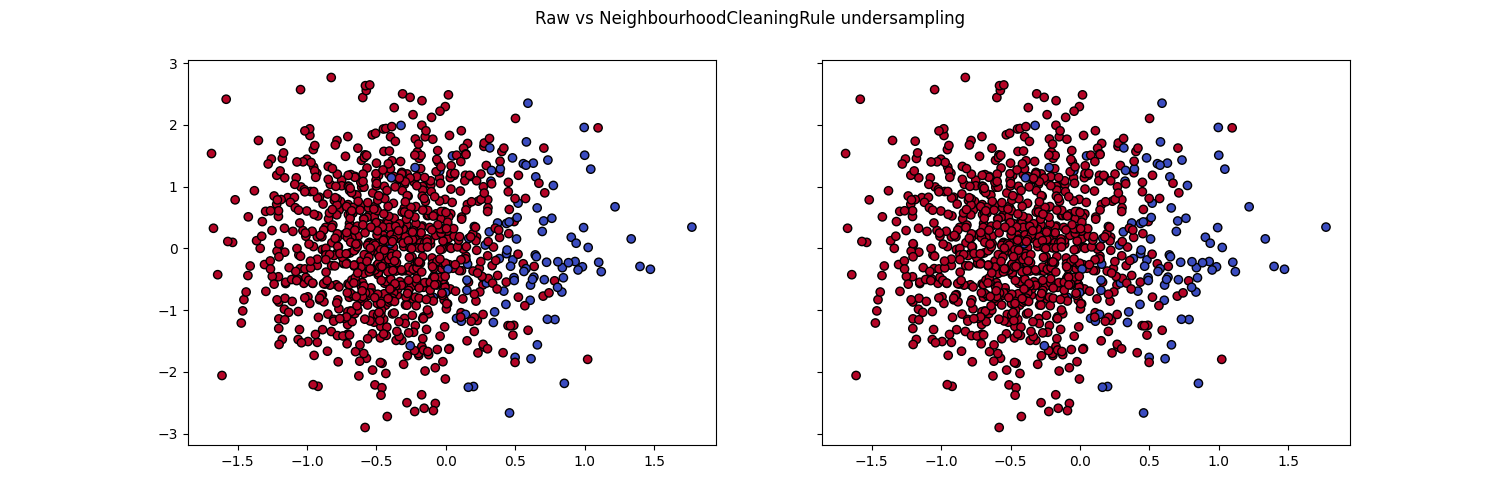
\includegraphics[width=0.6\textwidth]{images/Raw vs NeighbourhoodCleaningRule undersampling.png}
    \caption{NeighbourhoodCleaningRule örneği.}
    \label{fig:enter-label}
\end{figure}

\newpage

\subsection{Edited Nearest Neighbours (ENN)}
Başlangıçta, veri setindeki her bir örneğin sınıf etiketleri kontrol edilir. Her bir örnek için, bu örneğin sınıf etiketi ile k-NN (k en yakın komşu) algoritması kullanılarak belirlenen komşuların sınıf etiketleri karşılaştırılır. Eğer bir örnek, en azından biriyle komşu olmak üzere çoğunluk sınıfı etiketine sahip bir komşusu varsa ve kendisi azınlık sınıfına aitse, bu örnek veri setinden çıkarılır. Diğer örnekler de aynı şekilde incelenerek belirli bir kriteri sağlamayan örnekler kaldırılır ve daha dengeli bir alt örnekleme seti oluşturulur.

\subsubsection{Çalışma Adımları}

\begin{enumerate}
    \item İlk olarak, elimizdeki dengesiz veri seti hazırlanır. Bu veri seti hem çoğunluk sınıfı hem de azınlık sınıfı örneklerini içerir.
    \item ENN, her bir veri noktasının etrafındaki komşuları analiz eder. Bu işlem, k-NN algoritması ile yapılır. Amaç, her bir veri noktasının kendi sınıfında mı yoksa farklı bir sınıfta mı olduğunu anlamaktır.
    \item Her bir veri noktası, komşularıyla olan ilişkisine göre sınıflandırılır. Eğer bir veri noktası, komşularının çoğunluğu tarafından farklı bir sınıfa atanıyorsa, bu noktada bir sınıf karışıklığı yaşandığı kabul edilir.
    \item Eğer bir veri noktası, komşularının çoğu tarafından yanlış sınıflandırılıyorsa (örneğin, çoğunluk sınıfı bir örnek azınlık sınıfı gibi görünüyorsa), bu veri noktası veri setinden çıkarılır. Bu adım, özellikle çoğunluk sınıfı örneklerinin, azınlık sınıfı ile sınıf sınırlarında karışıklık yaratmasını engellemeye yöneliktir.
    \item ENN, yalnızca çoğunluk sınıfı değil, aynı zamanda azınlık sınıfı örnekleri üzerinde de çalışır. Eğer azınlık sınıfına ait bir veri noktası, k komşusunun çoğunluğu tarafından yanlış sınıflandırılıyorsa, bu nokta da veri setinden çıkarılabilir.
    \item Yukarıdaki adımlar sonucunda, yanlış sınıflandırılan veya gereksiz veri noktaları çıkarılarak veri seti yeniden oluşturulur.
\end{enumerate}

\subsubsection{Python Kod Implementasyonu}

\begin{lstlisting}[language=Python]
class EditedNearestNeighbors:
    def __init__(self, k_neighbors=3):
        self.k_neighbors = k_neighbors

    def fit_resample(self, X, y):
        class_counts = Counter(y)
        min_class_size = min(class_counts.values())
        classes = np.unique(y)
        
        X_resampled = []
        y_resampled = []

        for class_label in classes:
            X_class = X[y == class_label]
            
            knn = KNeighborsClassifier(n_neighbors=self.k_neighbors)
            knn.fit(X, y)
            
            neighbors = knn.kneighbors(X_class, return_distance=False)
            to_remove = []
            for i, idx in enumerate(neighbors):
                neighbor_labels = y[idx]
                if np.sum(neighbor_labels == class_label) <= (self.k_neighbors // 2):
                    to_remove.append(i)

            X_cleaned = np.delete(X_class, to_remove, axis=0)
            
            if X_cleaned.shape[0] > min_class_size:
                idx_to_keep = np.random.choice(X_cleaned.shape[0], min_class_size, replace=False)
                X_cleaned = X_cleaned[idx_to_keep]

            X_resampled.append(X_cleaned)
            y_resampled.append(np.full(X_cleaned.shape[0], class_label))

        X_resampled = np.vstack(X_resampled)
        y_resampled = np.hstack(y_resampled)

        return X_resampled, y_resampled
\end{lstlisting}

\begin{figure}[h]
    \centering
    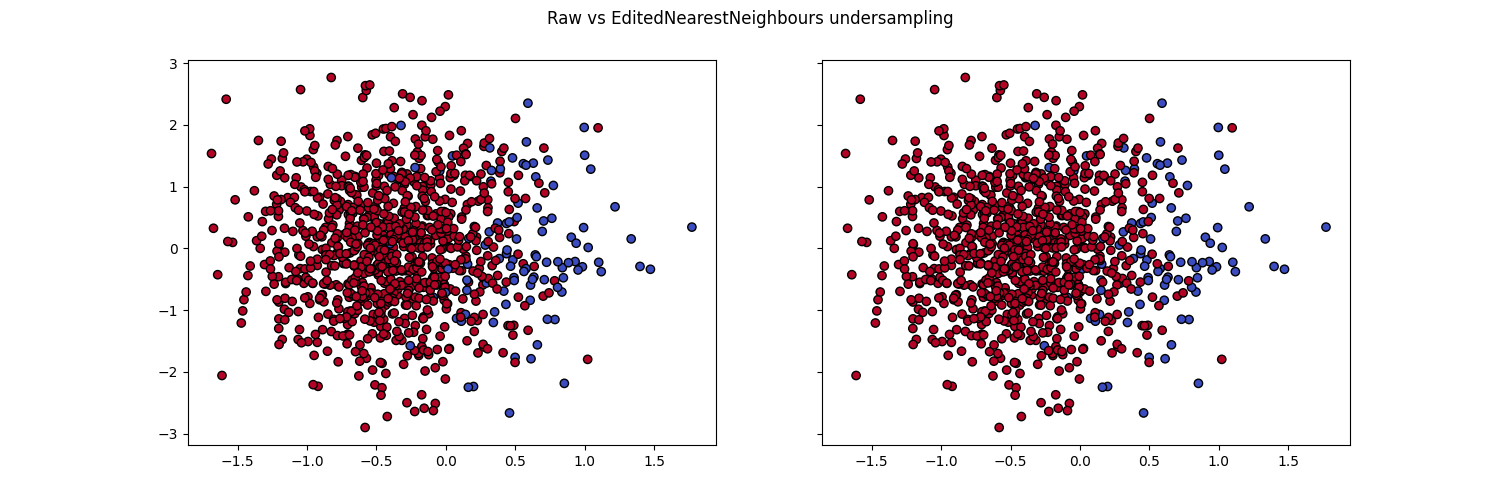
\includegraphics[width=0.6\textwidth]{images/Raw vs EditedNearestNeighbours undersampling.png}
    \caption{EditedNearestNeighbours örneği.}
    \label{fig:enter-label}
\end{figure}

\newpage

\subsection{Repeated Edited Nearest Neighbours (RENN)}
Başlangıçta, veri setindeki her bir örneğin sınıf etiketleri kontrol edilir. Her bir örnek için, bu örneğin sınıf etiketi ile k-NN (k en yakın komşu) algoritması kullanılarak belirlenen komşuların sınıf etiketleri karşılaştırılır. Eğer bir örnek, en azından biriyle komşu olmak üzere çoğunluk sınıfı etiketine sahip bir komşusu varsa ve kendisi azınlık sınıfına aitse, bu örnek veri setinden çıkarılır. Ardışık iterasyonlarla bu işlem tekrarlanarak, alt örnekleme seti güncellenir.

\subsubsection{Çalışma Adımları}

\begin{enumerate}
    \item Öncelikle elimizdeki dengesiz veri seti hazırlanır. Bu veri seti hem çoğunluk sınıfı hem de azınlık sınıfı örneklerini içerir.
    \item İlk adımda her bir veri noktası için en yakın k komşusu belirlenir. 
    \item Her bir veri noktası, komşularıyla karşılaştırılır. Eğer bir veri noktası komşularının çoğunluğu ile aynı sınıfta değilse, bu noktada bir sınıf sınırı karışıklığı olduğu kabul edilir.
    \item Eğer bir veri noktası komşularının çoğunluğu tarafından yanlış sınıflandırılıyorsa (örneğin, çoğunluk sınıfı bir örnek azınlık sınıfına ait gibi görünüyorsa), bu veri noktası veri setinden çıkarılır.
    \item RENN, bu temizleme işlemini yalnızca bir kez yapmaz. İlk temizlikten sonra, elde edilen yeni veri seti tekrar gözden geçirilir. Yeniden oluşturulan veri setinde, her bir veri noktası yeniden komşularıyla karşılaştırılır ve yanlış sınıflandırılan noktalar tekrar temizlenir. Bu süreç, veri setinde artık çıkarılacak veri kalmayana veya bir önceki temizleme adımı ile yeni adım arasında bir fark kalmayana kadar devam eder. Her döngüde yeni yanlış sınıflandırmalar tespit edilirse, bu noktalar çıkarılır. RENN bu tekrarlı temizleme sayesinde, daha temiz ve dengeli bir veri seti oluşturur.
    \item Temizlik işlemi birkaç iterasyondan sonra sona erer. İki ardışık temizleme işlemi arasında veri seti artık değişmediğinde, yani çıkarılacak yeni veri noktası kalmadığında algoritma durur.
\end{enumerate}

\subsubsection{Python Kod Implementasyonu}

\begin{lstlisting}[language=Python]
class RepeatedEditedNearestNeighbors:
    def __init__(self, k_neighbors=3):
        self.k_neighbors = k_neighbors

    def fit_resample(self, X, y):
        class_counts = Counter(y)
        min_class_size = min(class_counts.values())
        classes = np.unique(y)

        X_resampled = []
        y_resampled = []

        for class_label in classes:
            X_class = X[y == class_label]
            y_class = y[y == class_label]

            knn = KNeighborsClassifier(n_neighbors=self.k_neighbors)
            removed = True

            while removed:
                removed = False
                knn.fit(X_class, y_class)

                indices_to_keep = []
                for i in range(len(X_class)):
                    neighbors = knn.kneighbors([X_class[i]], return_distance=False)[0]
                    neighbors = neighbors[neighbors != i]
                    y_neighbors = y_class[neighbors]

                    if np.bincount(y_neighbors).argmax() == y_class[i]:
                        indices_to_keep.append(i)
                    else:
                        removed = True
                        
                X_class = X_class[indices_to_keep]
                y_class = y_class[indices_to_keep]

            if len(X_class) > min_class_size:
                indices_to_sample = np.random.choice(len(X_class), min_class_size, replace=False)
                X_class = X_class[indices_to_sample]
                y_class = y_class[indices_to_sample]

            X_resampled.append(X_class)
            y_resampled.append(y_class)

        X_resampled = np.vstack(X_resampled)
        y_resampled = np.hstack(y_resampled)

        return X_resampled, y_resampled
\end{lstlisting}

\newpage

\begin{figure}[h]
    \centering
    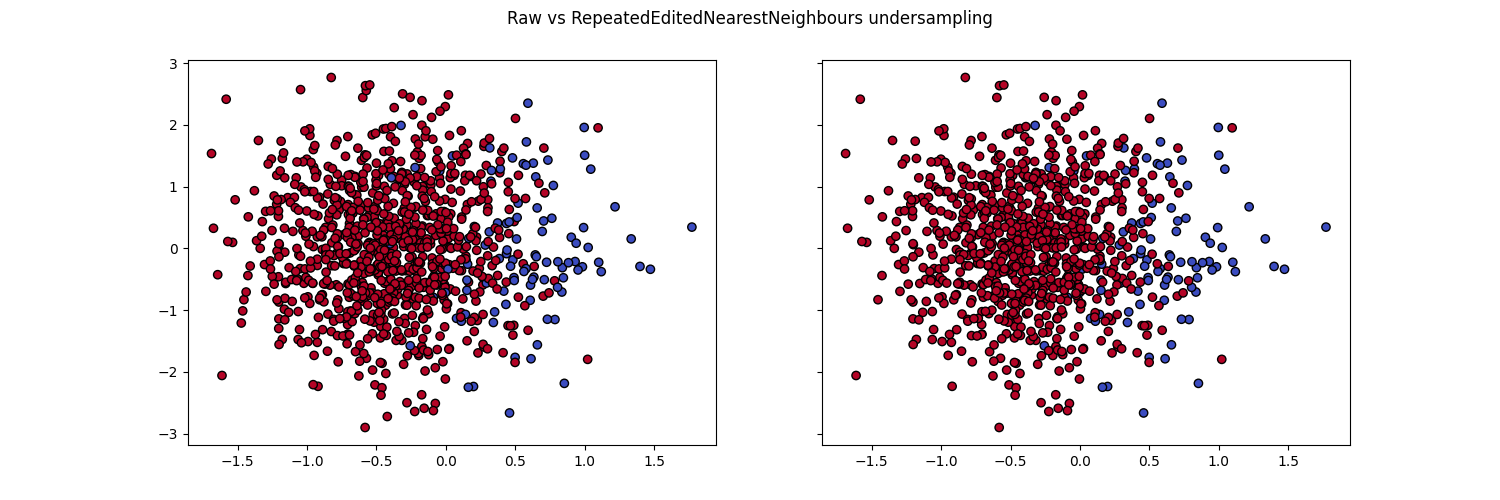
\includegraphics[width=0.6\textwidth]{images/Raw vs RepeatedEditedNearestNeighbours undersampling.png}
    \caption{RepeatedEditedNearestNeighbours örneği.}
    \label{fig:enter-label}
\end{figure}

\newpage

\subsection{AllKNN}
Veri setindeki her bir örnek için, k-NN algoritması kullanılarak örneğin etrafındaki komşular bulunur. Eğer bir örnek, en az k kadar komşusundan çoğunluk sınıfına aitse, bu örnek korunur. Eğer değilse, azınlık sınıfına aitse ve k değerinden az sayıda komşusu çoğunluk sınıfına aitse bu örnek veri setinden çıkarılır. Tüm örnekler bu şekilde kontrol edilerek, sınıf dengesizliği azaltmak için uygun olanlar belirlenir ve veri seti güncellenir.

\subsubsection{Çalışma Adımları}

\begin{enumerate}
    \item Veri setindeki her sınıfın gözlem sayıları hesaplanır ve hangi sınıfın azınlık (minority) ve hangi sınıfın çoğunluk (majority) olduğu belirlenir.
    \item AllKNN, veri setindeki her gözlem için KNN algoritmasını kullanarak bir komşuluk ilişkisi oluşturur. Bu yöntem, her gözlem için en yakın k komşusunu bulur.
    \item AllKNN’in ana amacı, sınıf sınırında veya komşuluk ilişkisine uymayan çoğunluk sınıfına ait örnekleri tespit etmektir. Bu örnekler:
    \begin{itemize}
        \item Eğer bir çoğunluk sınıfına ait örnek, komşularının büyük çoğunluğu azınlık sınıfına aitse, bu örnek sınıf sınırlarında bulunuyor olabilir ve modelin performansını kötü etkileyebilir. Bu tür gözlemler gereksiz olarak işaretlenir.
        \item Çok yakınında farklı sınıflara ait komşuları olan gözlemler, sınıf sınırlarında karışıklık yaratabilir ve bu da modelin tahmin performansını düşürebilir. Bu gözlemler çıkarılır.
    \end{itemize}
    \item KNN algoritmasıyla tespit edilen gereksiz çoğunluk sınıfı gözlemleri, veri setinden çıkarılır. Bu işlem, veri setinin dengesini sağlayarak azınlık sınıfının daha iyi temsil edilmesini sağlar. Veri setindeki gözlemler çıkarılırken gözlemlerin komşularına göre sınıf sınırında yer alıp almadıkları dikkate alınır. Çoğunluk sınıfındaki gözlemlerin sayısı, azınlık sınıfına göre belirli bir seviyeye indirgenir. Ancak azınlık sınıfı gözlemlerine dokunulmaz.
\end{enumerate}

\subsubsection{Python Kod Implementasyonu}

\begin{lstlisting}[language=Python]
class AllKNN:
    def __init__(self, k=3):
        self.k = k

    def fit_resample(self, X, y):
        nn = NearestNeighbors(n_neighbors=self.k + 1)
        nn.fit(X)

        distances, indices = nn.kneighbors(X)

        indices_to_remove = []

        for i in range(len(X)):
            neighbors = indices[i][1:]

            neighbor_labels = y[neighbors]
            if Counter(neighbor_labels).most_common(1)[0][0] != y[i]:
                indices_to_remove.append(i)

        mask = np.ones(len(X), dtype=bool)
        mask[indices_to_remove] = False
        X_resampled = X[mask]
        y_resampled = y[mask]

        class_counts = Counter(y_resampled)
        min_class_count = min(class_counts.values())

        X_balanced = []
        y_balanced = []

        for class_label in class_counts.keys():
            class_indices = np.where(y == class_label)[0]
            selected_indices = np.random.choice(
                class_indices, min_class_count, replace=False)
            X_balanced.append(X[selected_indices])
            y_balanced.append(y[selected_indices])

        X_balanced = np.vstack(X_balanced)
        y_balanced = np.hstack(y_balanced)
        return X_balanced, y_balanced
\end{lstlisting}

\begin{figure}[h]
    \centering
    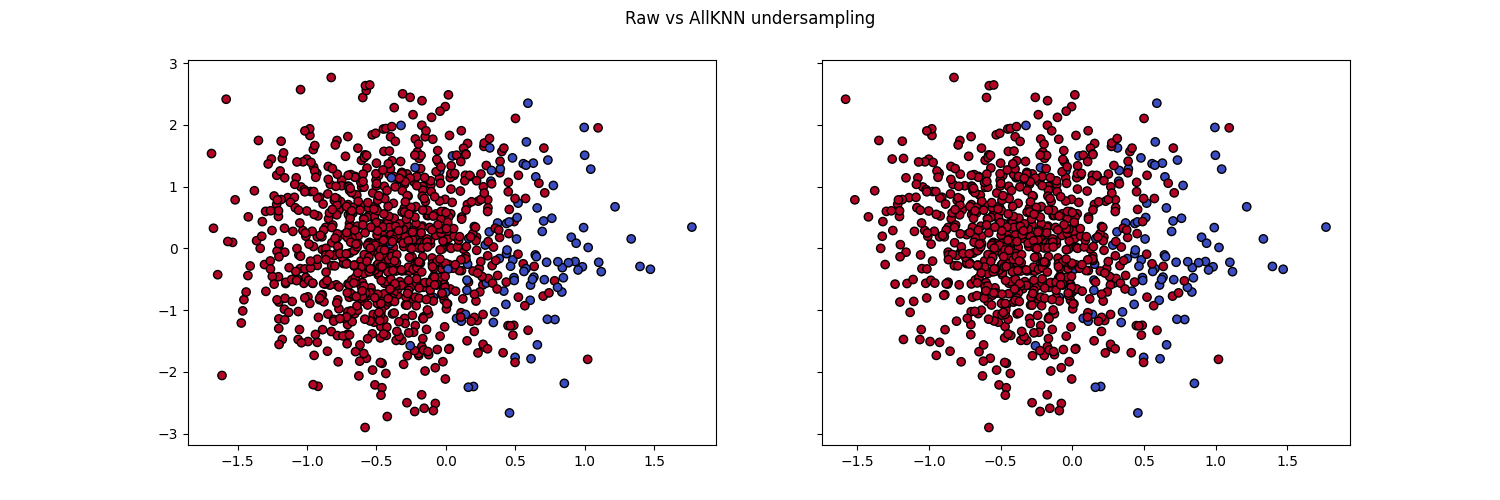
\includegraphics[width=1\textwidth]{images/Raw vs AllKNN undersampling.png}
    \caption{AllKNN örneği.}
    \label{fig:enter-label}
\end{figure}

\newpage

\subsection{Instance Hardness Threshold}
Her bir örnek için, bir sınıflandırma modeli (genellikle k-NN veya bir karar ağacı kullanılır) kullanılarak örneklerin zorluk seviyesi belirlenir. Bu, örneğin yanlış sınıflandırılma olasılığı veya belirsizlik derecesi gibi faktörlere dayanabilir. Bir eşik değeri belirlenir. Bu eşik değeri, seçilecek veya kaldırılacak örneklerin zorluk seviyesini belirler. Örnekler, belirlenen eşik değerine göre değerlendirilir. Eşik değerini geçen örnekler, model için zor olan veya belirsiz olan örnekler olarak kabul edilir ve kaldırılabilir veya azaltılabilir.

\subsubsection{Çalışma Adımları}

\begin{enumerate}
    \item İlk olarak, veri seti azınlık ve çoğunluk sınıflarını içerir.
    \item IHT, örneklerin zorluk seviyelerini belirlemek için bir sınıflandırma modeli kullanır. Genellikle bu amaçla lojistik regresyon, karar ağaçları veya destek vektör makineleri (SVM) gibi modeller tercih edilir. Veri setindeki her örnek için model eğitilir ve tahmin yapılır. Bu model, veri setindeki her bir örnek için hardness score (zorluk puanı) hesaplamak üzere kullanılır. Bu puan, modelin o örneği doğru sınıflandırıp sınıflandıramadığını gösterir.
    \item Zorluk puanı, her veri noktasının sınıflandırma modeline göre ne kadar zor sınıflandırıldığına dair bir ölçüdür. Bir örneğin zorluk puanı, modelin o örneği yanlış sınıflandırma olasılığına dayalıdır. Eğer model bir veri noktasını sınıflandırmakta zorlanıyorsa, o noktaya yüksek bir zorluk puanı atanır. Bu puanlar genellikle 0 ile 1 arasında bir değer alır:
    \begin{itemize}
        \item \textbf{1}: Örnek yanlış sınıflandırılmıştır ve zor bir örnektir.
        \item \textbf{0}: Örnek doğru sınıflandırılmıştır ve kolay bir örnektir.
    \end{itemize}
    \item Zorluk puanları hesaplandıktan sonra, hangi örneklerin veri setinden çıkarılacağına karar vermek için bir eşik değeri (threshold) belirlenir. Bu eşik değeri, zorluk puanı eşikten yüksek olan örneklerin çıkarılmasını sağlar. Eşik değeri ne kadar düşükse, daha fazla örnek çıkarılır. Çoğunluk sınıfından, zorluk puanı belirlenen eşiği aşan örnekler, veri setinden çıkarılır.
    \item Zorluk puanı belirlenen eşiğin üzerinde olan çoğunluk sınıfına ait örnekler, veri setinden çıkarılır. Bu işlem, veri setindeki gürültülü ve yanlış sınıflandırılmış örnekleri temizlemeyi hedefler. Böylece modelin yanlış öğrendiği veriler çıkarılmış olur. Zor örnekler genellikle sınıf sınırlarında yer alan, birbirine çok yakın ya da yanlış etiketlenmiş veriler olabilir.
    \item Çoğunluk sınıfından zor örnekler çıkarıldığında, veri seti daha dengeli hale gelir. Temizlenen veri seti, azınlık sınıfının daha iyi temsil edilmesini sağlar.
\end{enumerate}

\subsubsection{Python Kod Implementasyonu}

\begin{lstlisting}[language=Python]
from imblearn.under_sampling import InstanceHardnessThreshold
from sklearn.linear_model import LogisticRegression

iht = InstanceHardnessThreshold(random_state=0, sampling_strategy="auto", estimator=LogisticRegression())
X_resampled, y_resampled = iht.fit_resample(X_train, y_train)
\end{lstlisting}

\begin{figure}[h]
    \centering
    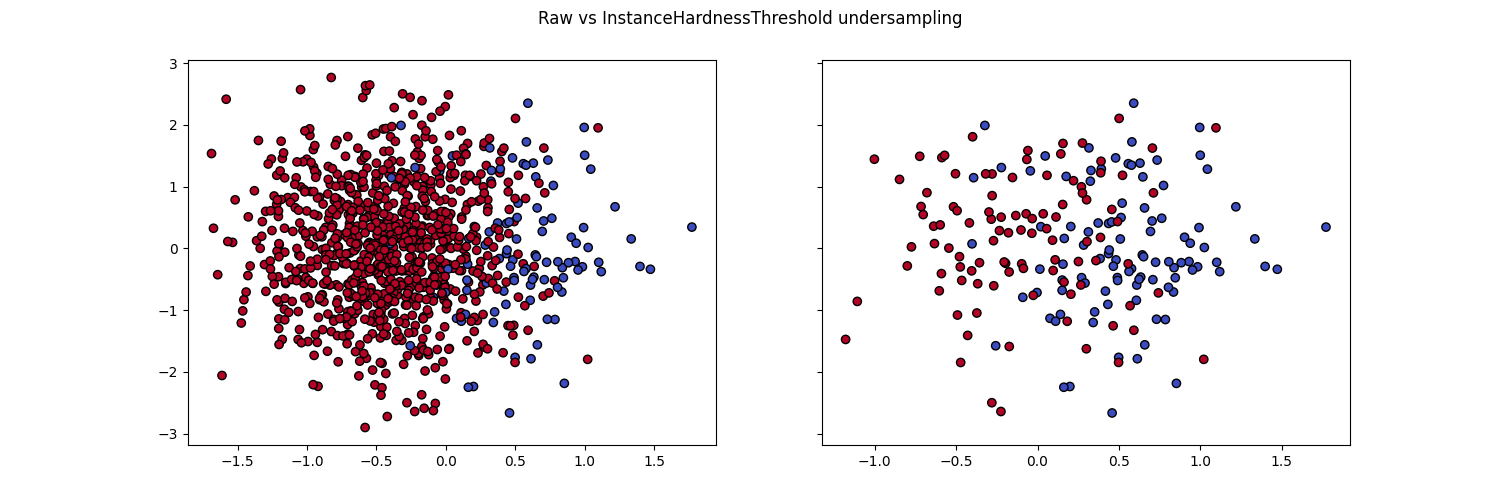
\includegraphics[width=1\textwidth]{images/Raw vs InstanceHardnessThreshold undersampling.png}
    \caption{InstanceHardnessThreshold örneği.}
    \label{fig:enter-label}
\end{figure}

\newpage